\documentclass[12pt,a4paper]{article}
\usepackage[utf8]{inputenc}
\usepackage[T1]{fontenc}
\usepackage{amsmath}
\usepackage{amssymb}
\usepackage{graphicx}
\usepackage{geometry}
\usepackage{booktabs}
\usepackage{hyperref}
\usepackage{float}
\usepackage{caption}
\usepackage{subcaption}
\usepackage{tikz}
\usetikzlibrary{shapes,arrows,positioning}

\geometry{margin=2.5cm}

\title{Stereo Vision and Visual Odometry \\ Project Report}
\author{AmirHossein Dashtban Namaghi}
\date{February 18, 2026}

\begin{document}

\maketitle

\section{Introduction}
This report details the implementation and evaluation of a comprehensive perception pipeline for autonomous vehicles, divided into two primary sections: **Stereo Depth Perception** (Part A) and **Stereo Visual Odometry** (Part B). The experiments were conducted on the KITTI Vision Benchmark Suite, using both the Scene Flow training set for depth evaluation and the Odometry dataset for trajectory estimation.

\section{Part A: Stereo Depth Perception}

\subsection{Pipeline Overview}
The stereo matching pipeline follows the traditional structure for rectified image pairs. The pipeline steps are visualized in Figure \ref{fig:stereo_pipeline}.

\begin{figure}[H]
    \centering
    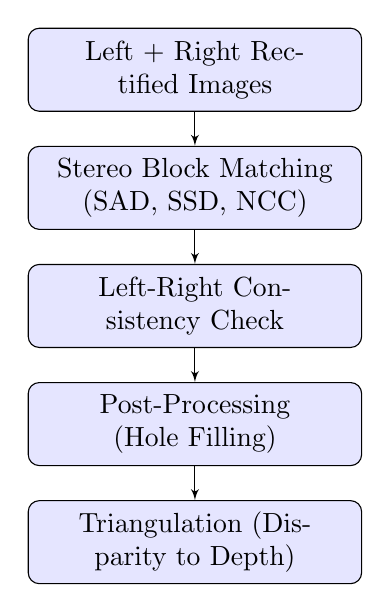
\begin{tikzpicture}[node distance=1.5cm, auto]
        \tikzstyle{block} = [rectangle, draw, fill=blue!10, text centered, rounded corners, minimum height=3em, text width=4cm]
        \tikzstyle{line} = [draw, -latex']
        
        \node [block] (input) {Left + Right Rectified Images};
        \node [block, below of=input] (matching) {Stereo Block Matching (SAD, SSD, NCC)};
        \node [block, below of=matching] (lrcheck) {Left-Right Consistency Check};
        \node [block, below of=lrcheck] (pp) {Post-Processing (Hole Filling)};
        \node [block, below of=pp] (tri) {Triangulation (Disparity to Depth)};
        
        \path [line] (input) -- (matching);
        \path [line] (matching) -- (lrcheck);
        \path [line] (lrcheck) -- (pp);
        \path [line] (pp) -- (tri);
    \end{tikzpicture}
    \caption{Stereo Depth Pipeline Diagram.}
    \label{fig:stereo_pipeline}
\end{figure}

\subsection{Matching Cost Functions}
The core of the stereo matching process is the block-matching algorithm with a Winner-Take-All (WTA) strategy. We implemented and compared three cost functions:
\begin{itemize}
    \item \textbf{Sum of Absolute Differences (SAD):} Simply the summed absolute pixel-wise differences within a window.
    \item \textbf{Sum of Squared Differences (SSD):} Squaring the differences penalizes large deviations more heavily.
    \item \textbf{Normalized Cross-Correlation (NCC):} Normalizes for local mean and variance. This is mathematically defined as:
    $$NCC(x,y,d) = \frac{\sum (I_L - \mu_L)(I_R - \mu_R)}{\sigma_L \sigma_R}$$
    It is significantly more robust to lighting variations but computationally more expensive without optimization.
\end{itemize}

\subsection{Calibration and Triangulation}
The focal length $f$ and baseline $B$ are extracted from the KITTI calibration files (e.g., \texttt{calib.txt}). The baseline is computed using the distance between the two rectified projection matrices' optical centers. For $P_2$ (Left) and $P_3$ (Right):
$$f = P_2[0, 0]$$
$$B = \frac{|P_3[0, 3] - P_2[0, 3]|}{f}$$
Triangulation then converts disparity $d$ into metric depth $Z$:
$$Z = \frac{f \cdot B}{d}$$

\subsection{Ablation Study (Depth)}
The study compared SAD, SSD, and NCC across window sizes of 5x5 and 11x11, averaged over 5 frames.

\begin{table}[H]
    \centering
    \begin{tabular}{@{}llcc@{}}
    \toprule
    Metric & Window & Avg Bad-Pixel Rate (\%) & Avg MAE \\ \midrule
    SAD    & 5x5    & 48.99                  & 11.84   \\
    SAD    & 11x11  & 34.59                  & 8.72    \\
    SSD    & 5x5    & 47.51                  & 11.55   \\
    SSD    & 11x11  & 32.78                  & 8.29    \\
    NCC    & 5x5    & 39.37                  & 8.85    \\
    \textbf{NCC} & \textbf{11x11} & \textbf{17.26} & \textbf{3.38} \\ \bottomrule
    \end{tabular}
    \caption{Ablation study for Stereo Depth.}
    \label{tab:ablation_depth}
\end{table}

\subsection{Failure Cases}
\begin{itemize}
    \item \textbf{Occlusions:} Pixels visible in the left image but blocked in the right create invalid disparities. These were handled by the Left-Right check and filled with horizontal streaking.
    \item \textbf{Repeated/Low Textures:} Road surfaces and glass reflectances create ambiguity in the NCC/SAD scores, leading to noisy "holes" or misalignments in the disparity map.
\end{itemize}

\begin{table}[H]
    \centering
    \begin{tabular}{@{}lccc@{} }
    \toprule
    KITTI Image ID & BPR (\%) & MAE (px) & Likely Failure Reason \\ \midrule
    000002\_10.png & 47.11 & 11.60 & Specularity on vehicles \\
    000006\_10.png & 45.67 & 8.63 & Occlusion boundaries \\
    000007\_10.png & 43.75 & 11.82 & Overexposure on road surface \\
    000010\_10.png & 42.44 & 8.30 & Repetitive foliage patterns \\ \bottomrule
    \end{tabular}
    \caption{Top 5 failure frames from Part A detected using \texttt{find\_failures.py}.}
    \label{tab:stereo_failures}
\end{table}

\subsection{Visual Results (10 Examples)}
The following figures showcase the Disparity and Depth maps for the first 10 frames of the Scene Flow dataset using the optimized NCC (11x11) algorithm.

\begin{figure}[H]
    \centering
    \begin{subfigure}{0.4\textwidth}
        \includegraphics[width=\textwidth]{/home/amirhossein/Music/project/results/result_00.png}
        \caption{Frame 00}
    \end{subfigure}
    \hfill
    \begin{subfigure}{0.4\textwidth}
        \includegraphics[width=\textwidth]{/home/amirhossein/Music/project/results/result_01.png}
        \caption{Frame 01}
    \end{subfigure}

    % \vspace{0.5cm}

    \begin{subfigure}{0.4\textwidth}
        \includegraphics[width=\textwidth]{/home/amirhossein/Music/project/results/result_02.png}
        \caption{Frame 02}
    \end{subfigure}
    \hfill
    \begin{subfigure}{0.4\textwidth}
        \includegraphics[width=\textwidth]{/home/amirhossein/Music/project/results/result_03.png}
        \caption{Frame 03}
    \end{subfigure}
    \caption{Qualitative Stereo Depth Results (Frames 00--03).}
    \label{fig:all_depth}
\end{figure}

\begin{figure}[H]
    \ContinuedFloat
    \centering
    \begin{subfigure}{0.4\textwidth}
        \includegraphics[width=\textwidth]{/home/amirhossein/Music/project/results/result_04.png}
        \caption{Frame 04}
    \end{subfigure}
    \hfill
    \begin{subfigure}{0.4\textwidth}
        \includegraphics[width=\textwidth]{/home/amirhossein/Music/project/results/result_05.png}
        \caption{Frame 05}
    \end{subfigure}

    % \vspace{0.5cm}

    \begin{subfigure}{0.4\textwidth}
        \includegraphics[width=\textwidth]{/home/amirhossein/Music/project/results/result_06.png}
        \caption{Frame 06}
    \end{subfigure}
    \hfill
    \begin{subfigure}{0.4\textwidth}
        \includegraphics[width=\textwidth]{/home/amirhossein/Music/project/results/result_07.png}
        \caption{Frame 07}
    \end{subfigure}
    \caption{Qualitative Stereo Depth Results (Frames 04--07, Continued).}
\end{figure}

\begin{figure}[H]
    \ContinuedFloat
    \centering
    \begin{subfigure}{0.4\textwidth}
        \includegraphics[width=\textwidth]{/home/amirhossein/Music/project/results/result_08.png}
        \caption{Frame 08}
    \end{subfigure}
    \hfill
    \begin{subfigure}{0.4\textwidth}
        \includegraphics[width=\textwidth]{/home/amirhossein/Music/project/results/result_09.png}
        \caption{Frame 09}
    \end{subfigure}
    \caption{Qualitative Stereo Depth Results (Frames 08--09, Continued).}
\end{figure}

\newpage

\section{Part B: Stereo Visual Odometry (VO)}

\subsection{Pipeline Overview}
The Visual Odometry pipeline uses ORB features tracked across frames to estimate the camera's pose $T \in SE(3)$. The simplified workflow is visualized in Figure \ref{fig:vo_pipeline}.

\begin{figure}[H]
    \centering
    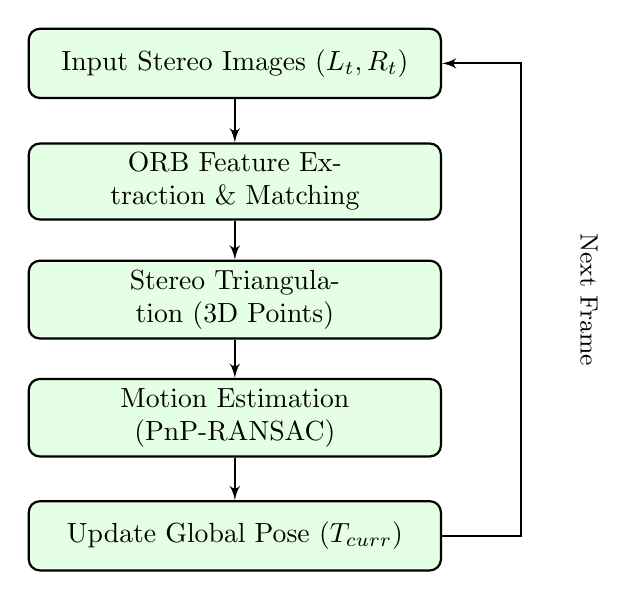
\begin{tikzpicture}[node distance=1.5cm, auto, thick]
        \tikzstyle{block} = [rectangle, draw, fill=green!10, text centered, rounded corners, minimum height=2.5em, text width=5cm]
        \tikzstyle{line} = [draw, -latex']
        
        \node [block] (input) {Input Stereo Images ($L_t, R_t$)};
        \node [block, below of=input] (feat) {ORB Feature Extraction \& Matching};
        \node [block, below of=feat] (tri) {Stereo Triangulation (3D Points)};
        \node [block, below of=tri] (ransac) {Motion Estimation (PnP-RANSAC)};
        \node [block, below of=ransac] (pose) {Update Global Pose ($T_{curr}$)};
        
        \path [line] (input) -- (feat);
        \path [line] (feat) -- (tri);
        \path [line] (tri) -- (ransac);
        \path [line] (ransac) -- (pose);
        
        % Feedback loop
        \draw [line] (pose.east) -- ++(1,0) |- (input.east);
        \node at (4.5, -3) [rotate=270, font=\small] {Next Frame};
    \end{tikzpicture}
    \caption{Simplified Stereo Visual Odometry Pipeline.}
    \label{fig:vo_pipeline}
\end{figure}

\begin{itemize}
    \item \textbf{Tracking}: Matches ORB features from $t \to t+1$ using Brute-Force Hamming matching.
    \item \textbf{Triangulation}: Matches features within the current stereo pair $(L_t, R_t)$ to obtain 3D world coordinates.
    \item \textbf{Motion Estimation}: Solves for the pose of frame $t+1$ using the PnP (Perspective-n-Point) algorithm on the $(P_{3D, t}, p_{2d, t+1})$ pairs.
\end{itemize}

\subsection{RANSAC and Robust Estimation}
RANSAC (Random Sample Consensus) is applied in a two-stage robust estimation process:
\begin{enumerate}
    \item \textbf{Geometric Consensus}: We first estimate the \textbf{Essential Matrix ($E$)} from 2D-2D temporal matches using RANSAC. This identifies the consistent epipolar geometry between frames.
    \item \textbf{Metric Motion}: We then perform \textbf{PnP RANSAC} using only the inliers from the first stage. This recovers the absolute scale via the previously triangulated 3D points.
\end{enumerate}
This hierarchical filtering is crucial for filtering out:
\begin{enumerate}
    \item Inaccurate feature matches on repetitive textures.
    \item Moving objects (which violate the static world assumption).
\end{enumerate}

\subsection{Evaluation on KITTI Sequences}
We evaluate our system on two sequences: Sequence 03 (City) and Sequence 01 (Highway, 1101 frames).

\begin{table}[H]
    \centering
    \begin{tabular}{@{}lccc@{}}
    \toprule
    Configuration & Sequence & Absolute Trajectory Error (m) & Relative Pose Error (m) \\ \midrule
    \textbf{Stereo VO (Full)} & 03 & \textbf{6.4498} & \textbf{0.0822} \\
    \textbf{Stereo VO (Full)} & 01 & 247.8687 & 1.9990 \\
    Ablation: No RANSAC & 03 & 2.51e11+ & N/A \\
    Ablation: No Scale  & 03 & 108.5530 & N/A \\ \bottomrule
    \end{tabular}
    \caption{Numerical evaluation for KITTI Sequences.}
    \label{tab:vo_eval}
\end{table}

\subsection{Ablation Study (VO Importance)}
The studies highlight two critical components:
\begin{itemize}
    \item \textbf{RANSAC Importance}: Without RANSAC, a single outlier match causes the pose estimation to explode immediately.
    \item \textbf{Stereo-based Scale Importance}: By using the stereo triangulation, we recover the **absolute metric scale**. Without it (monocular mode), the system defaults to an arbitrary scale factor of 1 per frame, leading to nearly 100 meters of cumulative scale drift on Seq 03.
\end{itemize}

\subsection{Feature Matches and Inliers (Seq 03)}
Figure \ref{fig:feature_matches_03} shows the ORB feature matches on Sequence 03.

\begin{figure}[H]
    \centering
    \begin{subfigure}{\textwidth}
        \includegraphics[width=\textwidth]{/home/amirhossein/Music/project/results_vo/vo_matches_seq03_f5_ransacTrue.png}
        \caption{S03 Frame 5}
    \end{subfigure}
    \begin{subfigure}{\textwidth}
        \includegraphics[width=\textwidth]{/home/amirhossein/Music/project/results_vo/vo_matches_seq03_f500_ransacTrue.png}
        \caption{S03 Frame 500}
    \end{subfigure}
    \caption{Temporal ORB Matching with RANSAC: Sequence 03.}
    \label{fig:feature_matches_03}
\end{figure}

\subsection{Large-Scale Trajectory Plot (Seq 03)}
\begin{figure}[H]
    \centering
    \includegraphics[width=0.8\textwidth]{/home/amirhossein/Music/project/results_vo/vo_traj_seq03_ransacTrue_scaleTrue.png}
    \caption{Trajectory for Sequence 03 (City loop).}
\end{figure}

\subsection{Results for Sequence 01 (Highway)}
Sequence 01 contains high-speed driving on a highway. Feature tracking is more challenging due to the distance of landmarks and high frame-to-frame displacement.

\begin{figure}[H]
    \centering
    \begin{subfigure}{\textwidth}
        \includegraphics[width=\textwidth]{/home/amirhossein/Music/project/results_vo/vo_matches_seq01_f5_ransacTrue.png}
        \caption{S01 Frame 5}
    \end{subfigure}
    \begin{subfigure}{\textwidth}
        \includegraphics[width=\textwidth]{/home/amirhossein/Music/project/results_vo/vo_matches_seq01_f500_ransacTrue.png}
        \caption{S01 Frame 500}
    \end{subfigure}
    \caption{Temporal ORB Matching: Sequence 01.}
    \label{fig:feature_matches_01}
\end{figure}

\begin{figure}[H]
    \centering
    \includegraphics[width=0.8\textwidth]{/home/amirhossein/Music/project/results_vo/vo_traj_seq01_ransacTrue_scaleTrue.png}
    \caption{Trajectory for Sequence 01 (Highway, 1101 Frames).}
\end{figure}


\end{document}
